%!TeX spellcheck = <brazil>
%%%%%%%%%%%%%%%%%%%%%%%%%%%%%%%%%%%%%%%%%
% Beamer Presentation
% LaTeX Template
% Version 1.0 (10/11/12)
%
% This template has been downloaded from:
% http://www.LaTeXTemplates.com
%
% License:
% CC BY-NC-SA 3.0 (http://creativecommons.org/licenses/by-nc-sa/3.0/)
%
%%%%%%%%%%%%%%%%%%%%%%%%%%%%%%%%%%%%%%%%%

%----------------------------------------------------------------------------------------
%	PACKAGES AND THEMES
%----------------------------------------------------------------------------------------

\documentclass{beamer}

\mode<presentation> {

\usetheme{Madrid}

\graphicspath{{./images/}} 



}

\usepackage{graphicx} % Allows including images
\usepackage{booktabs}
\usepackage[T1]{fontenc}
\usepackage[utf8]{inputenc}
\usepackage[english,brazil]{babel} % Allows the use of \toprule, \midrule and \bottomrule in tables

\usepackage{listings}
\usepackage{color}

\definecolor{dkgreen}{rgb}{0,0.6,0}
\definecolor{gray}{rgb}{0.5,0.5,0.5}
\definecolor{mauve}{rgb}{0.58,0,0.82}

\lstset{
	language=Java,
	aboveskip=1mm,
	belowskip=1mm,
	showstringspaces=false,
	columns=flexible,
	basicstyle={\small\ttfamily},
	numbers=none,
	numberstyle=\tiny\color{gray},
	keywordstyle=\color{blue},
	commentstyle=\color{dkgreen},
	stringstyle=\color{mauve},
	breaklines=false,
	breakatwhitespace=true,
	tabsize=1
}

%----------------------------------------------------------------------------------------
%	TITLE PAGE
%----------------------------------------------------------------------------------------

\title[TDD com Android]{Introdução A Testes de Unidade em Aplicativos Android} 
\author{Fernando Avanzo} % Your name
\institute[] 
{ % Your institution for the title page
\medskip
\textit{fernando.avanzo@gmail.com} % Your email address
}
\date{\today} % Date, can be changed to a custom date

\begin{document}

%-----------------------------------------------------------------------01
\begin{frame}
\titlepage % Print the title page as the first slide
\end{frame}

%-----------------------------------------------------------------------02
\begin{frame}
\frametitle{Overview} 
\tableofcontents % Throughout your presentation, if you choose to use \section{} and \subsection{} commands, these will automatically be printed on this slide as an overview of your presentation
\end{frame}

%------------------------------------------------
\section{Intro} % Sections can be created in order to organize your presentation into discrete blocks, all sections and subsections are automatically printed in the table of contents as an overview of the talk
%------------------------------------------------

\subsection{Tdd com Android} % A subsection can be created just before a set of slides with a common theme to further break down your presentation into chunks

%------------------------------------------------03
\begin{frame}
	\frametitle{Como funciona a estrutura de teste no android}
	Os projetos android criados a partir do Android Studio já vem com uma estrutura minima para a criação de testes automatizados
	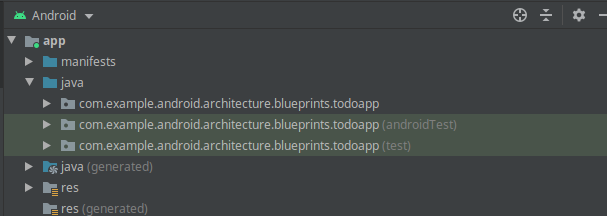
\includegraphics[scale=0.5]{test_structure_android}
	\newline Os arquivos são organizados da seguinte maneira
	\begin{itemize}
		\item diretório \textbf{main} onde fica todo código "funcional" do projeto
		\item diretório \textbf{test} onde fica todo código de teste que é executado localmente 
		\item diretório \textbf{androidTest} onde fica todo código de teste é executado no dispositivo
	\end{itemize}
	
\end{frame}

%------------------------------------------------04
\begin{frame}
	\frametitle{Caixa de ferramentas}
	Ao se escrever testes de unidade automatizados existe uma série de ferramentas úteis que auxiliam o workflow de trabalho. Abaixo vamos ver algumas:
	\newline 
	\begin{itemize}
		\item \href{https://junit.org/junit4/}{\textbf{Junit}} framework xUnit para escrita de testes de unidade
		\item \href{http://hamcrest.org/}{\textbf{Hamcrest}} biblioteca que permite a escrita de testes de forma mais idiomática, torna sua leitura mais fácil das pessoas entenderem.
		\item \href{https://developer.android.com/training/testing/set-up-project}
		{\textbf{AndroidX Test Library}} bibliotecas android que auxiliam na simulação de componentes do ciclo de vida da aplicação, (Context, Activitys, Fragments, etc)
		

	\end{itemize}
	
\end{frame}

%------------------------------------------------05
\begin{frame} [fragile]
	\frametitle{Configuração minima}
	Abaixo podemos ver qual o aspecto geral de um arquivo \textit{build.gradle} de um projeto orientado a testes.
	\newline 
	\begin{example}[\textit{build.gradle} default config]
		\begin{lstlisting}
			defaultConfig {
			applicationId "com.example.android..."
			minSdkVersion rootProject.minSdkVersion
			targetSdkVersion rootProject.targetSdkVersion
			versionCode 1
			versionName "1.0"
			testInstrumentationRunner 
				"androidx.test.runner.AndroidJUnitRunner"
			}
			
		\end{lstlisting}
	\end{example}
	
\end{frame}

%------------------------------------------------06
\begin{frame} [fragile]
	\frametitle{Configuração minima}
	
	\begin{example}[\textit{build.gradle} dependencias]
		\begin{lstlisting}
		// Dependencies for local unit tests
		testImplementation "junit:junit:$junitVersion"
		// AndroidX Test - Instrumented testing
		androidTestImplementation 
		"androidx.test.ext:junit:$androidXTestExtKotlinRunnerVersion"
		androidTestImplementation 
		"androidx.test.espresso:espresso-core:$espressoVersion"
		// AndroidX Test - JVM testing
		testImplementation 
		"androidx.test.ext:junit-ktx:$androidXTestKotlinRunnerVersion"
		testImplementation 
		"androidx.test:core-ktx:$androidXTestCoreVersion"
		testImplementation 
		"org.robolectric:robolectric:$robolectricVersion"
		// Other dependencies
		testImplementation 
		"org.hamcrest:hamcrest-all:$hamcrestVersion"
		
		\end{lstlisting}
	\end{example}
	
\end{frame}


%------------------------------------------------07
\begin{frame}
	\frametitle{Caso de Uso: ToDo App}
	Este é o aplicativo que vamos usar para estudar alguns casos práticos de teste de unidade
	\begin{columns}[c]
		
		\column{0.1\textwidth} % Left column and width
		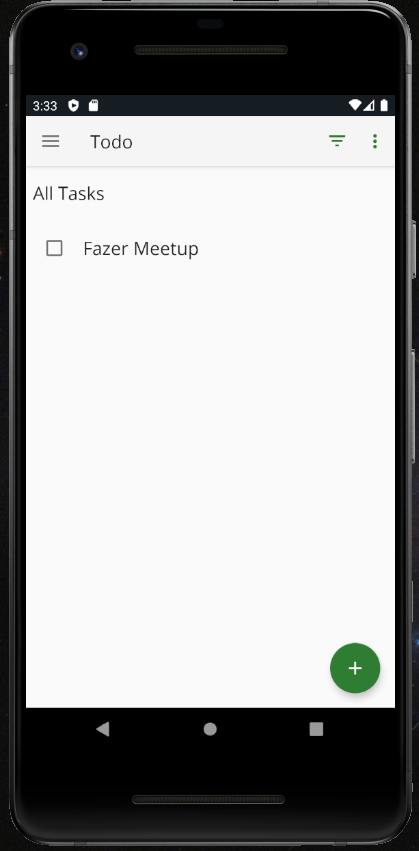
\includegraphics[scale=0.3]{toDoAppSample}
		\column{0.3\textwidth} % Right column and width
		Clássico aplicativo de lista tarefas, que permite que usuário adicione uma nova tarefa na lista, "check" aquelas que já foram concluídas, veja uma estatística simples de quantas atividades ele já concluiu e quantas ainda possui na lista.
		
	\end{columns}
	
\end{frame}

%---------------------------------------------------------------------------------08
\begin{frame}
	\frametitle{Escrevendo nosso primeiro teste}
	O app \textbf{ToDo} tem uma funcionalidade que permite que o usuário tenha uma métrica de quantas tarefas ele terminou e quantas ainda faltam, levando isso em conta, nosso primeiro teste deve verificar que \textbf{Dado} uma lista de tarefas, \textbf{Quando} a lista tem  apenas uma tarefa e ela não está completa, \textbf{Então} a porcentagem de tarefas ativas deve ser 100 e a porcentagem de tarefas completas deve ser 0
\end{frame}

%-----------------------------------------------------------------------------09
\begin{frame}[fragile]
	\frametitle{Escrevendo nosso primeiro teste}
		\begin{example}[Escrevendo o teste]
		\begin{lstlisting}
		class StatisticsUtilsTest {
		
			@Test
			fun getActiveAndCompletedStats_noCompleted_returnsHundredZero() 
			{
				val tasks = listOf(
				Task("title", "desc", isCompleted = false)
				)
				
				val result = getActiveAndCompletedStats(tasks)
				
				assertThat(result.activeTasksPercent, `is`(100f))
				assertThat(result.completedTasksPercent, `is`(0f))
			}
		}
		\end{lstlisting}
	\end{example}
	
\end{frame}

%--------------------------------------------------------------------------------10
\begin{frame}[fragile]
	\frametitle{Escrevendo nosso primeiro teste}
	\begin{example}[Escrevendo o codigo funcional]
		\begin{lstlisting}
		internal fun getActiveAndCompletedStats(tasks: List<Task>?)
		: StatsResult {
			val totalTasks = tasks!!.size
			val numberOfActiveTasks = tasks.count { it.isActive }
			return StatsResult(
				activeTasksPercent = 100f * 
					numberOfActiveTasks / tasks.size,
				completedTasksPercent = 100f * 
					(totalTasks - numberOfActiveTasks) / tasks.size)
		}
		\end{lstlisting}
	\end{example}
	
\end{frame}

%------------------------------------------------11
\begin{frame}
\frametitle{O que é TDD?}
TDD,(Test Drive Development), é uma prática de desenvolvimento de software que orienta a antes de escrever qualquer código funcional, escrever um código de teste, em seguida escrever o minimo de código funcional que faça o teste passar. Então trabalhar esse fluxo de forma incremental durante todo o processo de desenvolvimento.
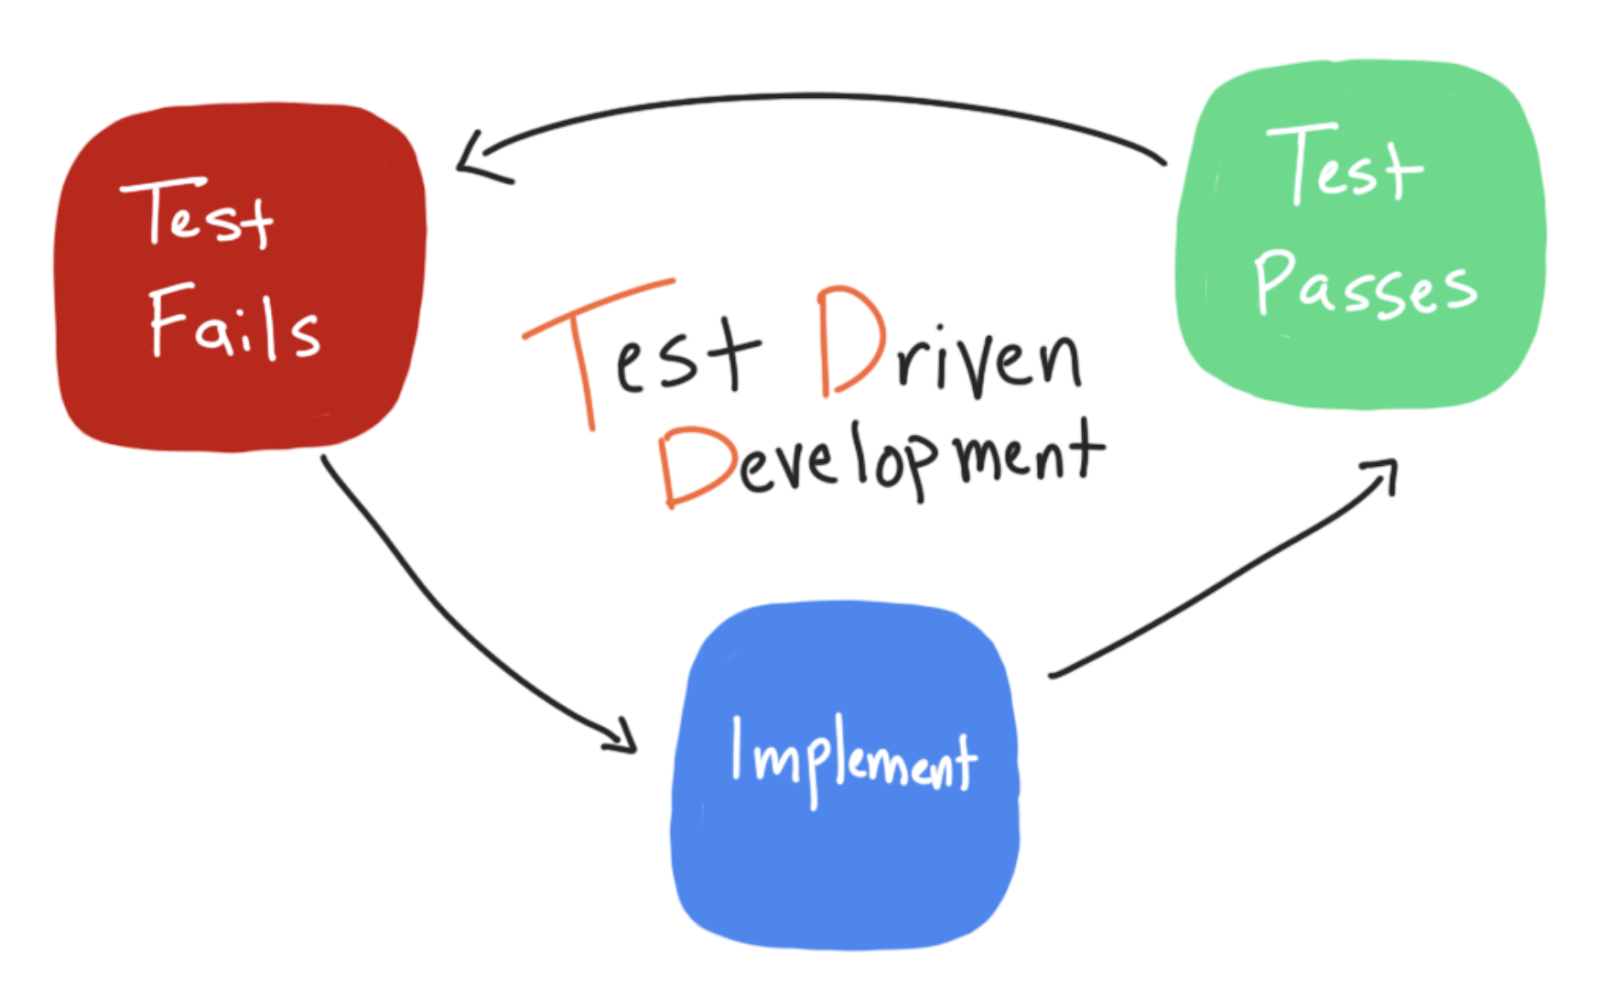
\includegraphics[scale=0.15]{tdd_diagram_flow}
 
\end{frame}

%------------------------------------------------12
\begin{frame}
	\frametitle{O Jeito de Pensar TDD}
	Um teste de unidade pode ser escrito em três etapas:
	\begin{block}{Dado (Given)}
		Qual é o estado atual? Nesta etapa os dados necessários para simular o estado atual da aplicação é fornecido.
	\end{block}
	
	\begin{block}{Quando (When)}
		Quando o estado muda? Nesta etapa o trecho de código (método, função, procedimento, etc..), que muda o estado é executado.
	\end{block}
	
	\begin{block}{Então (Then)}
		A resposta(saída), está certa? Nesta etapa é verificado se após o estado inicial ter sido alterado o resultado corresponde ao esperado.
	\end{block}
	
\end{frame}

%---------------------------------------------------------------------------------13
\begin{frame}
\frametitle{Caso de Uso: ToDo App}
Vamos ver um exemplo prático da abordagem GWT, (Given, When, Then) com o aplicativo ToDo
\newline \textbf{Cenário de uso:} O usuário tem uma lista de tarefas
\begin{itemize}
\item \textbf{Dado} que usuário possui uma lista de tarefas
\item \textbf{Quando} a lista de tarefas houver apenas uma tarefa e ela estiver completa.
\item \textbf{Então} a porcentagem de tarefas ativas deve ser 0 e a porcentagem de tarefas concluídas deve ser 100
\end{itemize}
\end{frame}

%---------------------------------------------------------------------------------14
\begin{frame}[fragile]
	\frametitle{Caso de Uso: ToDo App}
	\begin{example}[Escrevendo o teste]
		\begin{lstlisting}
		@Test
		fun getActiveAndCompletedStats_noActive_returnsZeroHundred() {
			//Given
			val tasks = listOf(Task("title", "desc", isCompleted = true))
			
			// When 
			val result = getActiveAndCompletedStats(tasks)
		
			// Then 
			assertThat(result.activeTasksPercent, `is`(0f))
			assertThat(result.completedTasksPercent, `is`(100f))
		}
		\end{lstlisting}
	\end{example}
\end{frame}

%---------------------------------------------------------------------------------15
\begin{frame}[fragile]
	\frametitle{Caso de Uso: ToDo App}
	\begin{example}[Escrevendo o codigo funcional]
		\begin{lstlisting}
		internal fun getActiveAndCompletedStats(tasks: List<Task>?)
		: StatsResult {
		
			val totalTasks = tasks!!.size
			val numberOfActiveTasks = tasks.count { it.isActive }
			val activePercent = 100 * numberOfActiveTasks / totalTasks
			val completePercent = 100 * 
				(totalTasks - numberOfActiveTasks) / totalTasks
		
			return StatsResult(
				activeTasksPercent = activePercent.toFloat(),
				completedTasksPercent = completePercent.toFloat())
		}
		\end{lstlisting}
	\end{example}
\end{frame}

%---------------------------------------------------------------------------------16
\begin{frame}
	\frametitle{Caso de Uso: ToDo App}
	Cenário de Bug: Temos uma lista nula ou vazia
	\begin{itemize}
		\item \textbf{Dado} que uma lista nula ou vazia é enviada
		\item \textbf{Quando} a lista de tarefas for processada.
		\item \textbf{Então} a porcentagem de tarefas ativas e concluídas deve ser 0
	\end{itemize}
\end{frame}

%--------------------------------------------------------------------------------17
\begin{frame}[fragile]
	\frametitle{Caso de Uso: ToDo App}
	\begin{example}[Escrevendo o teste]
		\begin{lstlisting}
		@Test
		fun getActiveAndCompletedStats_error_returnsZeros() {
			//Given
			val tasks = null
		
			// When
			val result = getActiveAndCompletedStats(null)
		
			//Then
			assertThat(result.activeTasksPercent, `is`(0f))
			assertThat(result.completedTasksPercent, `is`(0f))
		}
		\end{lstlisting}
	\end{example}
\end{frame}

%---------------------------------------------------------------------------------18
\begin{frame}[fragile]
	\frametitle{Caso de Uso: ToDo App}
	\begin{example}[Escrevendo o codigo funcional]
		\begin{lstlisting}
		internal fun getActiveAndCompletedStats(tasks: List<Task>?)
		: StatsResult {
			return if (tasks == null || tasks.isEmpty()) {
				StatsResult(0f, 0f)
			} else {
				val totalTasks = tasks.size
				val numberOfActiveTasks = tasks.count { it.isActive }
				StatsResult(
					activeTasksPercent = 100f *
						 numberOfActiveTasks / tasks.size,
					completedTasksPercent = 100f * 
						(totalTasks - numberOfActiveTasks) / tasks.size)
			}
		}
		\end{lstlisting}
	\end{example}
\end{frame}

%------------------------------------------------19
\begin{frame}
\frametitle{References}
\footnotesize{
\begin{thebibliography}{99} % Beamer does not support BibTeX so references must be inserted manually as below
\bibitem[Smith, 2012]{p1} John Smith (2012)
\newblock Title of the publication
\newblock \emph{Journal Name} 12(3), 45 -- 678.
\end{thebibliography}
}
\end{frame}

%------------------------------------------------20

\begin{frame}
\Huge{\centerline{The End}}
\end{frame}

%----------------------------------------------------------------------------------------

\end{document} 